\section{Teori}
\label{sec:joel_o-theory}
För att analysera beroenden till paket i npm behövs först en robust beskrvning av hur dessa beroenden fungerar ges. Här presenteras hur npm implementerar beroenden samt den graf-modell som används vid analysen. För att kunna svara på frågeställning \ref{joel_o-fs:3} definieras även de relevanta kvalitetsfaktorerna.

\subsection{Beroenden i npm}
Projekt som använder sig av npm sparar sina egenskaper i json-filen \texttt{package.json}\cite{npm-package.json}. Detta gäller både projekt som i sig ska publiceras som paket i npm-registret och projekt som endast använder sig av npm-paket.
Denna fil beskriver ett projekts beroenden. \texttt{package.json} även innehåller fält så som namn, version och licens som är relevanta då projektet ska publiceras på npm.

Npm delar upp beroenden i flera kategorier. De kategorier som har undersökts i detta arbete är \textit{dependencies} och \textit{devDependencies}. \textit{dependencies} är de beroenden som det färdiga projektet kommer att förlita sig på. Dessa paket innehåller funktionalitet som används då den färdiga Javascript-applikationen körs. \textit{devDependencies} innehåller beroenden till paket som endast är nödvändiga under utvecklingen av projektet. Dessa innefattar exempelvis testramverk eller verktyg för kodanalys. I \texttt{package.json} finns även möjlighet att ange \textit{peerDependencies}, \textit{bundledDependencies} och \textit{optionalDependencies}. Dessa har dock lämnats utanför denna undersökning eftersom de sällan används och har liten påverkan på resultatet.

I \texttt{package.json} anges varje beroende som en samling där namn på paket kopplas till vilken version av paketet beroendet hänvisar till. Se exempel i figur \ref{fig:package.json}. Versionsnummer anges med tre siffror separerade med punkter.\cite{npm-semver} Npm tillåter också dessa versionsreferenser att skrivas på flera olika sätt för att matcha flera olika versionsnummer. Exempelvis betyder \texttt{*} eller \texttt{x} att samtliga versioner är accepterade, \texttt{latest} endast den senaste versionen och \texttt{1.2.3} endast version 1.2.3. Det finns även mer komplicerade mönster som specifierar vissa omfång av versioner samt tecknen \texttt{\^} och {\textasciitilde} som gör skillnad på de tre olika siffrorna i versionsnumret. För en fullständig beskrivning av olika versionsreferenser se \cite{npm-semver}. I \texttt{package.json} tillåts även beroenden till paket utanför npm-ekosystemet. För dessa är versionsnumret istället en länk till det paket beroendet refererar till.

\lstset{language=Java}
\begin{figure}[h]
  \center
  \begin{minipage}[c]{5cm}
    \begin{lstlisting}
...,
"dependencies": {
    "util": "0.10.3"
  },
  "devDependencies": {
    "mocha": "~1.21.4",
    "zuul": "~3.10.0",
    "zuul-ngrok": "^4.0.0"
  },
...
    \end{lstlisting}
  \end{minipage}
  \caption{Beroenden i \texttt{package.json} för version 1.4.1 av paketet \textit{assert}.\cite{npm-assert}}
  \label{fig:package.json}
\end{figure}

\subsection{Grafmodell för beroenden}
En tydlig modell över hur beroenden mellan paket i npm vävs samman till ett stort nätverk ges av en riktad graf. I denna graf motsvarar noderna olika paket. För att modellen ska överensstämma med npm-registret behöver olika versioner av samma paket behandlas som olika noder, eftersom beroenden är specifierade mot specifika versioner. Beroenden från ett paket kan också ändras mellan versioner, vilket gör att ett paket ej kan generaliseras till en nod. Kanterna mellan noderna modellerar beroenden med riktning från det beroende paketet till det paket som det beror på. Exempel på denna struktur kan ses i figur \ref{fig:beroende-graf-cykel}.

I de fall ett paket specifierar flera accepterade versioner i ett beroende har i denna undersökning endast den senaste versionen använts. Detta är konsekvent med npm:s beteende då paket hämtas. Det anses därför ointressant för att behandla detta som flera olika beroenden.

\begin{figure}
  \captionsetup{justification=centering}
  \centering
  \begin{subfigure}[t]{.5\textwidth}
    \begin{minipage}[t][8cm][b]{0,5\textwidth}
      \vspace*{\fill}
        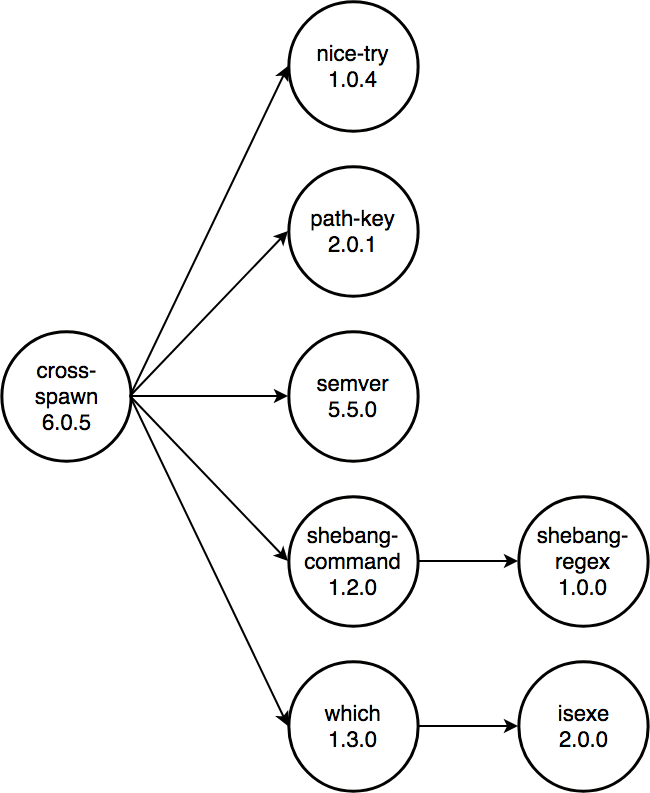
\includegraphics[scale=0.27]{dependency_graph}
      \vspace*{\fill}
    \end{minipage}
    \caption{Beroenden från version 6.0.5 av paketet \textit{cross-spawn}}
    \label{fig:beroende-graf}
  \end{subfigure}%
  \begin{subfigure}[t]{.5\textwidth}
    \begin{minipage}[t][8cm][b]{0,5\textwidth}
      \vspace*{\fill}
      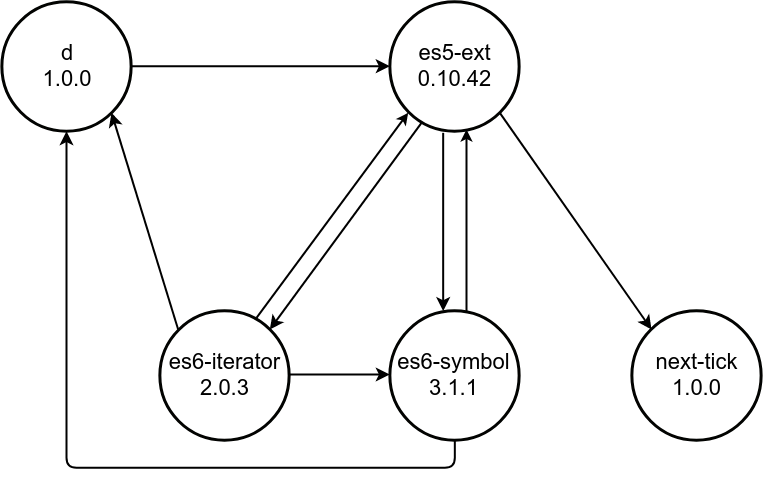
\includegraphics[scale=0.27]{dependency_graph_cycle}
      \vspace*{\fill}
    \end{minipage}
    \caption{Cykliska beroenden}
    \label{fig:beroende-graf-cykel}
  \end{subfigure}
  \caption{Exempel på grafmodeller över beroenden}
  \label{fig:grafmodell}
\end{figure}

Något som gör denna modell något speciellt komplex att arbeta med är att npm ej ställer några krav på att beroenden inte får bilda cykler. Det kan tyckas ointuitivt att detta kan fungera. Beroende är dock endast krav på att ett visst paket måste ha hämtats. När en cykel följs och ett paket nås som redan har passerats behöver detta inte hämtas igen och därmed skapar dessa cykler inga större problem. Exempel på flera sådana cirkulära beroenden kan ses i figur \ref{fig:beroende-graf-cykel};

\subsection{GitHub}
De olika Javascript-projekt som undersöks i detta arbete hämtas från plattformen GitHub. För projekt som ligger under en open-source-licens är all källkod tillgänglig att hämtas från GitHubs server. Detta innefattar filen \texttt{package.json} som är av stort intresse för denna undersökning. För att npm ska kunna använda \texttt{package.json} korrekt behöver denna fil vara placerad i projektets rotmapp. Detta underlättar analysen, då ett antagande om sökvägen till \texttt{package.json} i projektets mappstruktur kan göras.

Projekt på GitHub refereras till genom en unik kombination av ägarens användarnamn och projektets namn. Med denna information kan för ett visst projekt filen \texttt{package.json} hittas på adressen

\texttt{raw.githubusercontent.com/användarnamn/projektnamn/master/package.json}.

Om denna adress ej pekar på någon fil för ett visst projekt, och \texttt{package.json} därmed inte existerar, tyder det på att projektet ej använder sig av npm för pakethantering.

GitHub erbjuder ett sök-api för som kan användas för att hitta ett urval av projekt att analysera.\cite{github-api} Detta tillåter sökningar efter projekt skrivna på ett visst programmeringsspråk och med ett visst antal strjärnor. Stjärnor är systemet GitHub använder för att ranka omtyckta paket. Användare kan stjärnmarkera projekt de tycker om och därmed ger antalet stjärnor ett projekt har tilldelats en bra bild över hur populärt paketet är.

\subsection{Säkerhet och tillförlitlighet}
%TODO
Definition säkerhet

Definition tillförlitlighet (reliability) baserad runt MTTF i kontexten npm-paket
